\subsection{Login} \label{sec:Login}
Dette afsnit indeholder en gennemgang af den grafiske brugergrænseflade, design og implementering af 'Login' viewet i Rambøll Tilsyn.

\subsubsection{Design}
På Figur \ref{fig:LoginSekvens} ses sekvensdiagrammet for 'Login' viewet til Rambøll Tilsyn.
\begin{figure}[H] % (alternativt [H])
	\centering
	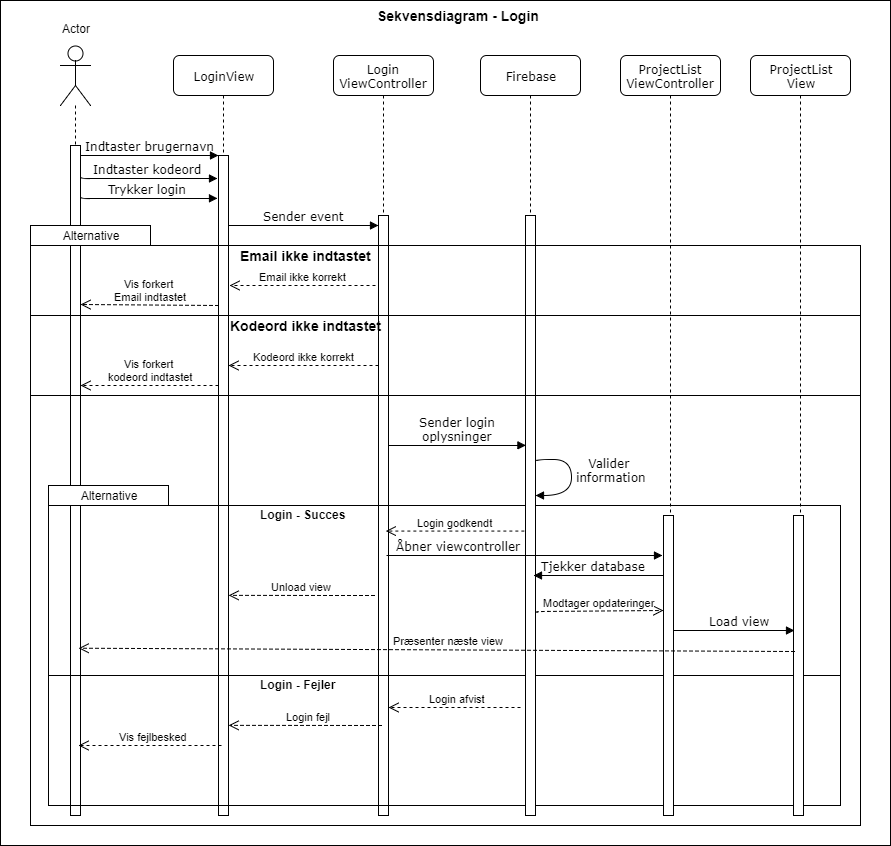
\includegraphics[height=15cm, width=15cm]{../ArkitekturDesign/Design/Login/LoginSekvensDiagram}
	\caption{Sekvensdiagram for 'Login' i Rambøll Tilsyn.}
	\label{fig:LoginSekvens}
\end{figure}

\clearpage

\subsubsection{Grafisk brugergrænseflade}
I 'Login' viewet er der lavet felter til at bruger indtaster sit brugernavn og kodeord. Se Figur \ref{fig:OpretBrugerView}
\begin{figure}[H] % (alternativt [H])
	\centering
	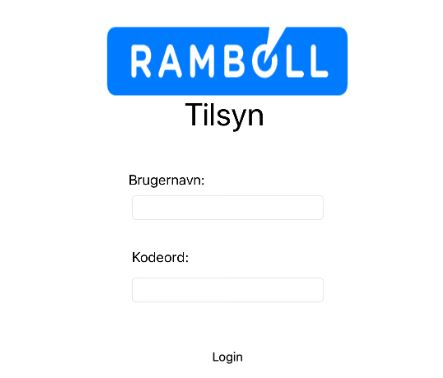
\includegraphics[height=12cm, width=10cm]{../ArkitekturDesign/Design/Login/LoginView}
	\caption{'Login' viewet som det er implementeret i Rambøll Tilsyn.}
	\label{fig:LoginView}
\end{figure}

\clearpage

\subsubsection{Implementering}
I dette afsnit vil der blive beskrevet funktionaliteten for de vigtigste funktioner i koden tilhørende 'Login' viewet.

På Figur \ref{fig:Checkifusersigned} ses funktionen for CheckIfUserSignedIn().
\begin{figure}[H] % (alternativt [H])
	\centering
	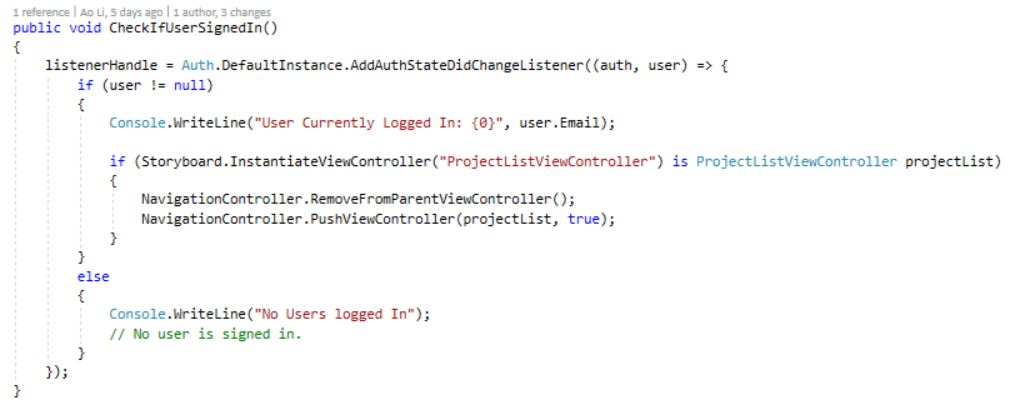
\includegraphics[height=8cm, width=15cm]{../ArkitekturDesign/Design/Login/Checkifusersigned}
	\caption{Kode snip - CheckIfUserSignedIn() fra LoginViewController.cs}
	\label{fig:Checkifusersigned}
\end{figure}
Først tjekker funktionen Firebases default instance og ser om, der er en bruger, som er logget ind. \\
Er der en bruger logget ind, hoppes log ind over, og projekt listen bliver vist. \\
Ellers udskriver den at ingen bruger er logget ind.

På Figur \ref{fig:ViewDidLoadLogin} ses funktionen for ViewDidLoad().
\begin{figure}[H] % (alternativt [H])
	\centering
	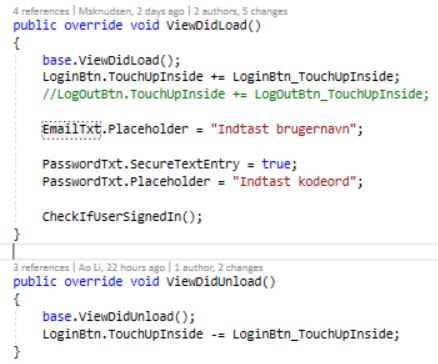
\includegraphics[height=7cm, width=12cm]{../ArkitekturDesign/Design/Login/ViewDidLoad}
	\caption{Kode snip - ViewDidLoad() fra LoginViewController.cs}
	\label{fig:ViewDidLoadLogin}
\end{figure}

\clearpage

I ViewDidLoad delegeres en eventhandler\cite{Event} til LoginBtn.TouchUpInside. \\
Den indsætter placeholders i tekstfelterne e-mail og kodeord. Derudover maskerer den inputs i kodeords tekstfelt.
I ViewDidUnload fjernes eventhandleren igen, da dette er en god kode skik for at undgå memory leak\cite{Memory}.

På Figur \ref{fig:LoginBtn} ses funktionen for LoginBtn.TouchUpInside().
\begin{figure}[H] % (alternativt [H])
	\centering
	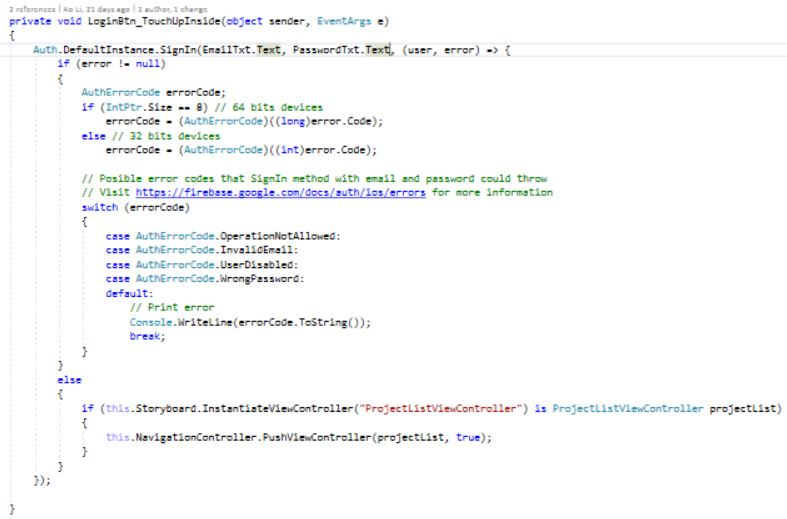
\includegraphics[height=10cm, width=18cm]{../ArkitekturDesign/Design/Login/LoginBtn}
	\caption{Kode snip - LoginBtn.TouchUpInside() fra LoginViewController.cs}
	\label{fig:LoginBtn}
\end{figure}
LoginBtn.TouchUpInside tager default instance af Firebase Auth, kalder SignIn metoden for denne instance og indsætter de to parameter skrevet i 'Login' viewet. \\
Efterfølgende valideres resultatet af log ind forsøget. Hvis der ingen fejl er, altså at e-mail og kodeord er korrekt, så vil projekt listen blive vist. \\
Der kan i switch-casen implementeres fejlhåndtering af diverse fejlkoder. 


\clearpage